\documentclass[10pt]{beamer}

%\usepackage{lmodern}
%\usepackage[labelformat=empty,font=scriptsize,skip=0pt,justification=justified,singlelinecheck=false]{caption}

%\usepackage{paralist}
%\usepackage{amsmath}% http://ctan.org/pkg/amsmath
%\usepackage{amsfonts}% http://ctan.org/pkg/amsfonts

%\usepackage[font=scriptsize]{caption}

%\usepackage{hyperref}
\usepackage{amssymb,amsmath,amsfonts,eurosym,geometry,graphicx,caption,color,setspace,
comment,footmisc,caption,pdflscape,array}
\usepackage{booktabs}   % for nice tables
\usepackage{multirow}
%\usepackage[round]{natbib}
\setbeamertemplate{caption}[numbered]
\usepackage[export]{adjustbox}

\usepackage[skip=1pt]{caption}
%\usepackage[capposition=top]{floatrow}

%\usepackage[caption = false]{subfig}
%\usepackage{floatrow}
\usepackage[capposition=bottom]{floatrow}

\usepackage{graphicx}
\usepackage{tabularx}
%\usepackage{threeparttable}
\usepackage{float}
\usepackage{mwe}
%\usepackage{subfig}
%\usepackage{polyglossia}
\usepackage{subcaption}
\setlength{\abovecaptionskip}{2pt}
%\usepackage[tight,TABTOPCAP]{subfigure}
\usepackage[round]{natbib}

\usepackage{multicol, latexsym, amsmath, amssymb}

\usepackage[normalem]{ulem}
\useunder{\uline}{\ul}{}
\usepackage{booktabs,caption}
\usepackage[flushleft]{threeparttable}

\usepackage{graphics}

\usepackage{longtable}

\usepackage{float}

\usepackage{amsbsy} %boldsymbol

%%in case of outdated TEX Live
\usepackage{lmodern}

\usepackage{appendixnumberbeamer}

%\graphicspath{{figures/}{../figures/}{D:/Presentations\figures/}}
\usepackage[normalem]{ulem}

\mode<presentation> {

% The Beamer class comes with a number of default slide themes
% which change the colors and layouts of slides. Below this is a list
% of all the themes, uncomment each in turn to see what they look like.

%\usetheme{default}
%\usetheme{AnnArbor}
%\usetheme{Antibes}
%\usetheme{Bergen}
%\usetheme{Berkeley}
%\usetheme{Berlin}
%\usetheme{Boadilla}
%\usetheme{CambridgeUS}
%\usetheme{Copenhagen}
%\usetheme{Darmstadt}
%\usetheme{Dresden}
%\usetheme{Frankfurt}
%\usetheme{Goettingen}
%\usetheme{Hannover}
%\usetheme{Ilmenau}
%\usetheme{JuanLesPins}
%\usetheme{Luebeck}
\usetheme{Madrid}
%\usetheme{Malmoe}
%\usetheme{Marburg}
%\usetheme{Montpellier}
%\usetheme{PaloAlto}
%\usetheme{Pittsburgh}
%\usetheme{Rochester}
%\usetheme{Singapore}
%\usetheme{Szeged}
%\usetheme{Warsaw}

% As well as themes, the Beamer class has a number of color themes
% for any slide theme. Uncomment each of these in turn to see how it
% changes the colors of your current slide theme.

%\usecolortheme{albatross}
%\usecolortheme{beaver}
%\usecolortheme{beetle}
%\usecolortheme{crane}
%\usecolortheme{dolphin}
%\usecolortheme{dove}
%\usecolortheme{fly}
%\usecolortheme{lily}
%\usecolortheme{orchid}
%\usecolortheme{rose}
%\usecolortheme{seagull}
%\usecolortheme{seahorse}
%\usecolortheme{whale}
%\usecolortheme{wolverine}

%\setbeamertemplate{footline} % To remove the footer line in all slides uncomment this line
%\setbeamertemplate{footline}[page number] % To replace the footer line in all slides with a simple slide count uncomment this line

%\setbeamertemplate{navigation symbols}{} % To remove the navigation symbols from the bottom of all slides uncomment this line
}
\usecolortheme{seahorse}

\usepackage{graphicx} % Allows including images
\usepackage{booktabs} % Allows the use of \toprule, \midrule and \bottomrule in tables

\usepackage{arydshln} %can use hdashline

\setbeamertemplate{footnote}{%
  \hangpara{2em}{1}%
  \makebox[2em][l]{\insertfootnotemark}\footnotesize\insertfootnotetext\par%
}
%----------------------------------------------------------------------------------------
%	TITLE PAGE
%----------------------------------------------------------------------------------------

\title[Task Specialization \& NF Wage Gap]{Task Specialization and the Native-Foreign Wage Gap: \\ Evidence from Worker-level Data} % The short title appears at the bottom of every slide, the full title is only on the title page

\author{Eduard Storm} % Your name
\institute[estorm@carleton.edu]
 % Your institution as it will appear on the bottom of every slide, may be shorthand to save space
{
	
	
	\medskip 
	
	Department of Economics \\  
	Carleton College \\ % Your institution for the title page
%	\textit{estorm@carleton.edu} % Your email address
	
	\bigskip
	
	 Job Market Paper Presentation for: \\
		\smallskip
	\textit{RWI Essen}
}


\date{January 21, 2021} % Date, can be changed to a custom date

\begin{document}

\begin{frame}
\titlepage % Print the title page as the first slide
\end{frame}



%----------------------------------------------------------------------------------------
%	PRESENTATION SLIDES
%----------------------------------------------------------------------------------------

%------------------------------------------------

%\begin{frame} 
%\frametitle{Overview}

%\textbf{Core theme in a nutshell}
%\bigskip
%\begin{itemize}
%\item [$\Rightarrow$] Refined measurement of Skills using detailed Task information and how they translate into Wage differences
%\end{itemize}
 
%\bigskip
 
%\begin{enumerate}
%\item Comparison of individual (self-reported) vs commonly used occupation-level task data (derived from external assessments of labor market experts)
%\item Implications of variation in individual tasks on the Native-Foreign Wage Gap with an emphasis on distributional effects
%\end{enumerate} 
 
%\bigskip
 
%\begin{itemize}
%\item Primary data set
%	\begin{itemize}
%	\item German employment surveys, assembled by the Federal Institute for Vocational Education (BIBB), the Institute of Employment Research (IAB) and the Federal Institute of Occupational Safety and Health (BAuA)
%	\item Provide self-reported information about job-related activities at the individual level
%	\end{itemize}
%\end{itemize}
 
 
%\end{frame}

%------------------------------------------------
%------------------------------------------------



\begin{frame} 
	\frametitle{Motivation}
	
	
	\begin{figure}[H]
		\centering
		\begin{minipage}{0.90\textwidth} % choose width suitably
			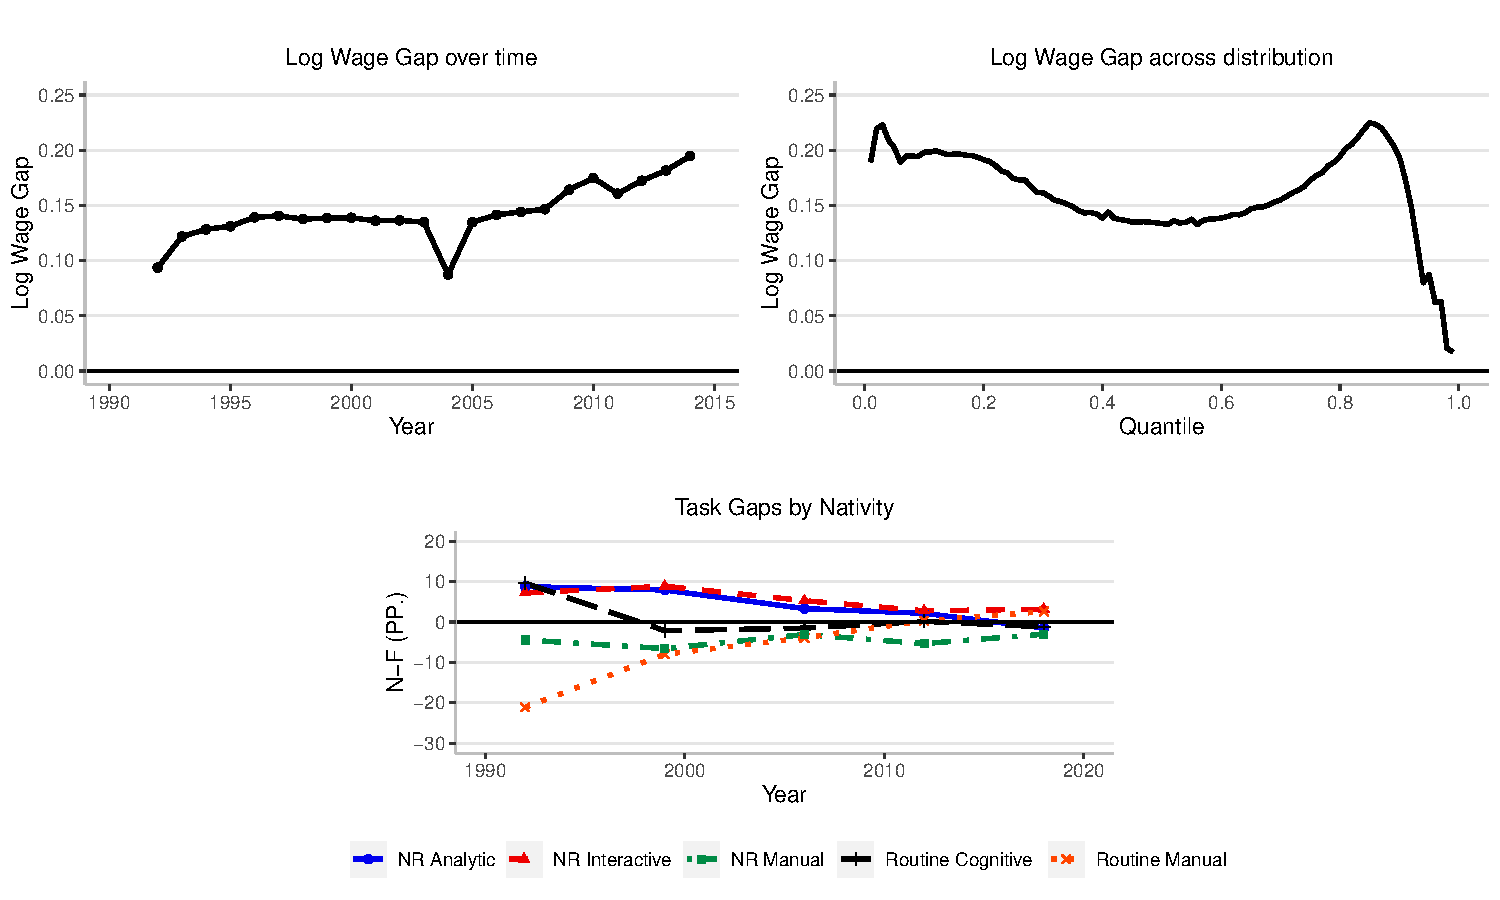
\includegraphics[width=0.90\linewidth]{wgap_tgap}
			\caption{  Native-Foreign (NF) Wage \& Task Gap in Germany, 1992-2018 \\ 
				\medskip \centering \tiny Source: SIAB-R 7514, BIBB/IAB/BAuA \label{fig:wage_gap}}
			{\footnotesize \tiny NOTE. \textemdash ``NR'' stands for Non-Routine Activities. NR Analytic and NR Interactive can be subsumed under \textit{Abstract} tasks, involving lots of problem-solving skills. Routine Cognitive and Routine Manual can be subsumed under \textit{Routine} tasks, characterized by various repetitive steps. NR \textit{Manual} involves activities requiring hand-eye coordination, which are difficult to automate.  \par}
			%{\caption  {Contributions of Task Variation Within Occupations to the explained Native-Foreign Wage Gap with base task group Routine Manual, 1992-2018 \label{fig:wgap_within_baserm}}}
		\end{minipage}
	\end{figure}
	

\end{frame}

%------------------------------------------------
\begin{frame} 
	\frametitle{Motivation}
	
	
	\begin{itemize}
		\item If F workers assimilate in terms of educational outcomes\footnote[frame]{Omitted in this presentation, see paper for details.} and tasks, then why do we not observe a convergence in wages?
	\end{itemize}
	
\end{frame}

%------------------------------------------------
\begin{frame}
	\frametitle{Contributions}
	
	\begin{enumerate}
		\item \textbf{Variation in Tasks at worker-level predictive of the NF Wage Gap}
		\begin{itemize}
			\item Robust to inclusion of Education and Experience measures
			\medskip
			\item[$\Rightarrow$] Challenges identifying assumptions in structural models in which N \& F with similar education-experience profile are assumed to be perfect substitutes (e.g., \textit{D'Amuri, Ottaviano \& Peri 2010})
		\end{itemize} 
		
		\smallskip
		
		\item \textbf{RIF Decomposition applied to Migration Context}
		\begin{itemize}
			\item Idiosyncratic differences pronounced among high-wage earners 
			\item Contribute up to 25\% to explained wage gap
			\medskip
			\item[$\Rightarrow$] Conventional decomposition methods such as Oaxaca-Blinder (OB) understate the impact of tasks on wage gaps
		\end{itemize} 
		
		\smallskip
		
		\item \textbf{Between-Occupation vs Within-Occupation Contributions}
		\begin{itemize}
			\item Occupational segregation: $\geq 70\%$ 
			\item \underline{Within-Occupation specialization}: $\geq 10\%$   %only for high-wage earners
			\medskip
			\item[$\Rightarrow$] Focus on occupational segregation alone understates degree of task specialization between N \& F (e.g., \textit{Peri \& Sparber 2009, 2011})
		\end{itemize} 
		
		
		
	\end{enumerate}
	
	
	
\end{frame}

%------------------------------------------------
\begin{frame} 
	\frametitle{Data}
	
	\begin{itemize}	
		\item German employment surveys provided by BIBB/IAB/BAuA\footnote[frame]{BIBB = Federal Institute for Vocational Education, IAB = Institute of Employment Research, BAuA = Federal Institute of Occupational Safety and Health} 
		\begin{itemize}
			\item[-] Key: Information on \textit{self-reported} tasks by workers (1992 - 2018)
		\end{itemize}
		
	\end{itemize}
	
	
	\begin{figure}[H]
		\begin{adjustbox}{addcode={\begin{minipage}{\width}}{\caption{From Activities to Tasks: Construction of the Task Content \label{fig:tasks_creation}
				}\end{minipage}},center}
			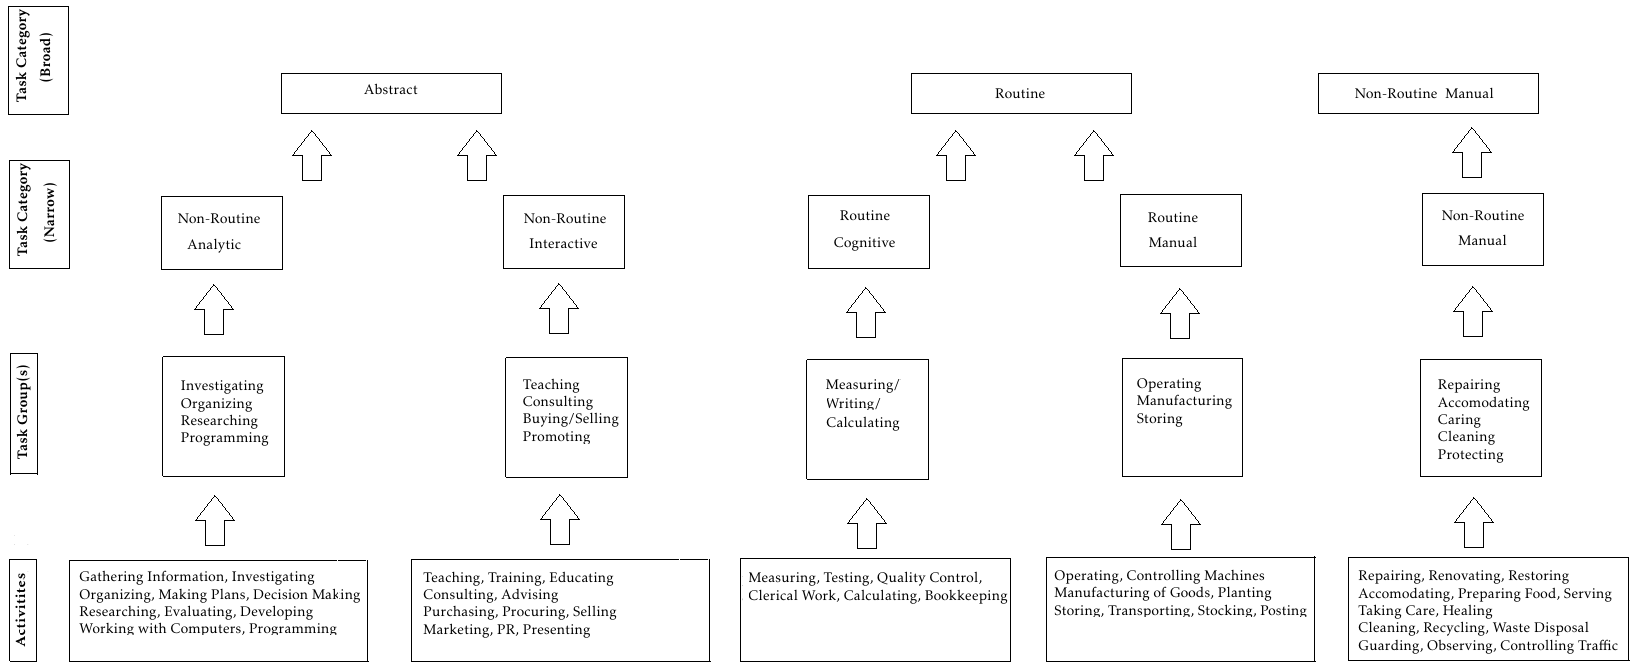
\includegraphics[scale=.36]{task_aggregation_illustration_FINAL}%
		\end{adjustbox}
	\end{figure}
	
	%,rotate=90
	
\end{frame}

%------------------------------------------------
\begin{frame} 
	\frametitle{Data}
	
	
	
	%\bigskip
	
	\begin{itemize}
		\item \textbf{\underline{Measuring individual task content}}: Compute relative importance of task category $j$ for individual $i$ at time $t$\footnote[frame]{following \textit{Antonczyk, Fitzenberger, and Leuschner (2009)}}  
	\end{itemize}
	
	\medskip
	
	
	\begin{equation} \label{task_def2}
	T_{ijt} = \frac{\text{No. of activities performed by i in task category j at time t}}{\text{Total no. of activitites by i across \textit{all} j's at time t}}
	\end{equation}
	
	\bigskip
	
	
	Note:
	\begin{itemize}
		\item $T_{ijt} \in [0,1]$ $\forall j$\\
		\item $\sum_{J} T_{ijt} = 1$\\
	\end{itemize}
	
\end{frame}

%------------------------------------------------
\begin{frame} 
	\frametitle{Data}
	
	
	\begin{itemize}
		\item \textbf{\underline{Measuring occupational task content}}:  Collect $T_{ijt}$ for all $N_{o}$ workers employed in occupation $o$ at time $t$
	\end{itemize}
	
	\begin{equation} \label{task_def_occ}
	T_{jot} = \frac{1}{N_{ot}} \sum_{i} T_{ijt_{o_{sub}}} 
	\end{equation} 
	
	
	\begin{itemize}
		\item [$-$]  $sub \in ({o_{90}, o_{00}})$ \\
		\begin{itemize}
			\item  $o_{90}$ = sub-sample 1992-99 \\
			\item  $o_{00}$ = sub-sample 2006-18 \\
		\end{itemize}
	\end{itemize}
	
	\bigskip
	
	Note:
	\begin{itemize}
		\item $T_{jo} \in [0,1]$ $\forall j$\\
		\item $\sum_{J} T_{jo} = 1$\\
	\end{itemize}
	
	
\end{frame}

%------------------------------------------------
\begin{frame} 
	\frametitle{Methodology}
	
	\textbf{Main Analysis: Recentered Influence Function (RIF) Decomposition}
	
	
	\begin{itemize}
		\item Conventional Oaxaca-Blinder (OB) Decomposition for groups $g=N, F$:   
	\end{itemize}
	
	\begin{equation} \label{ob_decomp}
	\Longrightarrow	\overline{w}_N - \overline{w}_F =  \underbrace{(\overline{X}_F - \overline{X}_N) \hat{\beta}_N}_\text{Explained Part} + \underbrace{\overline{X}_F(\hat{\beta}_N - \hat{\beta}_F)}_\text{Unexplained Part}
	\end{equation} 
	
	\bigskip
	
	\begin{itemize}
		\item \textbf{What I do:} Generalize OB by applying it along the wage distribution and replace mean wages with corresponding RIF by $g=N, F$ at decile $\tau$:
	\end{itemize}
	
	\begin{equation} \label{rif_decomp}
	\Longrightarrow 	RIF_{\tau}^{N} - RIF_{\tau}^{F} =  \underbrace{(\overline{X}_{\tau}^{F} - \overline{X}_{\tau}^{N}) \hat{\beta}_{\tau}^{N}}_\text{Explained Wage Gap} + \underbrace{\overline{X}_{\tau}^{F}(\hat{\beta}_{\tau}^{N} - \hat{\beta}_{\tau}^{F})}_\text{Unexplained Wage Gap}
	\end{equation} 
	
	
	
	
\end{frame}

%------------------------------------------------

\begin{frame} 
	\frametitle{Methodology: Recentered Influence Function (RIF) Decomposition}
	
	\begin{itemize}
		\item Following \textit{Firpo, Fortin \& Lemieux (2009)}, construct an RIF based on:
	\end{itemize}
	
	\begin{equation} \label{rif_def}
	RIF_{g}(w_{g},p_{\tau}) = \underbrace{\frac{\tau - I(w_{g} \leq p_{\tau})}{f_{w_{g}} (p_{\tau})}}_\text{Influence Function (IF)} + \underbrace{p_{\tau}}_\text{Recentered (R)}
	\end{equation} 
	
	
	\begin{itemize}
		\item[$-$]$g=N, F$ \\
		\item[$-$]$p_{\tau}$: Log Hourly Real Wage at decile $\tau = 0.1, ..., 0.9$
		\item[$-$]$I(w_{g} \leq p_{\tau})$: Indicator suggesting if observed wage for $g=N, F$ falls below decile $p_{\tau}$  \\
		\item[$-$]${f_{w_{g}} (p_{\tau})}$: Marginal density of $w_{g}$ associated with $p_{\tau}$ \\
		
		
	\end{itemize}
	
	\bigskip
	
	%	\begin{itemize}
	%		\item Generalization of the conventional Oaxaca-Blinder (OB) Decomposition :
	%	\end{itemize}
	
	
	%	\begin{equation} \label{rif_decomp}
	%	RIF_{\tau}^{N} - RIF_{\tau}^{F} =  \underbrace{(\overline{X}_{\tau}^{F} - \overline{X}_{\tau}^{N}) \hat{\beta}_{\tau}^{N}}_\text{Explained Wage Gap} + \underbrace{\overline{X}_{\tau}^{F}(\hat{\beta}_{\tau}^{N} - \hat{\beta}_{\tau}^{F})}_\text{Unexplained Wage Gap}
	%	\end{equation} 
	
	
\end{frame}

%------------------------------------------------



\begin{frame}[label=regression]  
	\frametitle{Methodology}
	
	
	\begin{itemize}
		\item Perform quantile regressions by replacing the original dependent variable ($ln\ w_{it}$) with its corresponding RIF:
	\end{itemize}
	
	
	\begin{equation} \label{6}
	\widehat{RIF_{g}(ln\ w_{it},p_{\tau}| \boldsymbol{T_{}}, \boldsymbol{X_{}}      ) } = \alpha + \boldsymbol{ \beta_{1} } \boldsymbol{T_{it}} + \boldsymbol{ \beta_{2} } \boldsymbol{T_{ot}} + \boldsymbol{ \gamma } \boldsymbol{X_{it}} + \delta_t + \lambda_r + \eta_s  + \epsilon_{it}
	\end{equation} 
	
	\begin{itemize}
		\item[$-$]$\boldsymbol{T_{it}} = \big(T_{i1t}, T_{i2t}, ..., T_{iJt} \big)$: Task category $j$ performed by $i$ at time $t$ \\
		\item[$-$]$\boldsymbol{T_{ot}} = \big(T_{1o}, T_{2ot}, ..., T_{Jot} \big)$: Task category $j$ performed in occupation $o$ \\
		\item[$-$]$\textbf{X}_{it}$: Controls \\
		\item[$-$]$\delta_t$, $\lambda_r$, $\eta_s$: Time, Region, Sector dummies
	\end{itemize} 
	
\hyperlink{occ_spec}{\beamergotobutton{Occupational Segregation}} \\
\hyperlink{wi_spec}{\beamergotobutton{Within-Occupation Specialization}} 	
	
	
	
\end{frame}

%------------------------------------------------
\begin{frame}
	\frametitle{Key Results RIF Decomposition: Explained Wage Gap}
	
	
%	\begin{figure}[H]
%		\begin{minipage}{0.95\textwidth} % choose width suitably
%			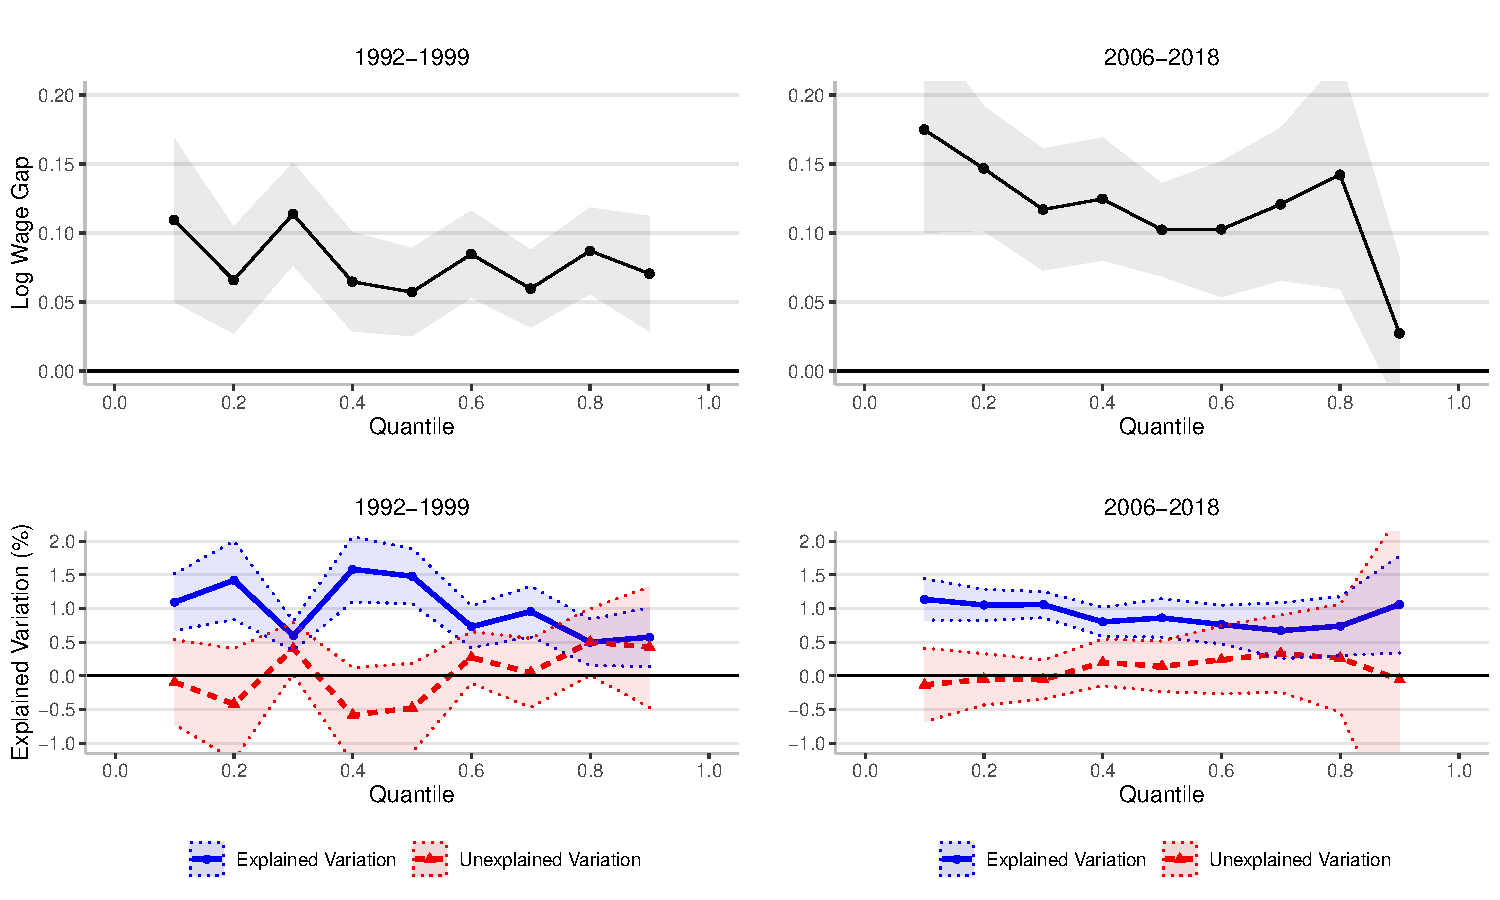
\includegraphics[scale=0.4]{nfgap_t} \\
%			{\footnotesize \tiny NOTE. \textemdash Point estimates are displayed with a 95\% Confidence Interval. \par}
%			\caption{\centering German Native-Foreign Wage Gap by sub-samples, 1992-2018 \label{fig:wgap_subs}}
%		\end{minipage}
%	\end{figure}
%	
	
	
\end{frame}

%------------------------------------------------
\begin{frame} 
	\frametitle{Assessment of Relative Importance of Task Measures}
	
	
	Visual evidence from Figure (\ref{fig:wgap_subs}) combined with eq. \eqref{rif_decomp} implies for most $\tau$: \\
	
	
	\begin{center}
		\begin{equation} \label{rif_decomp_mod}
		\begin{aligned}
		RIF_{\tau}^{N} - RIF_{\tau}^{F} &=  \underbrace{(\overline{X}_{\tau}^{F} - \overline{X}_{\tau}^{N}) \hat{\beta}_{\tau}^{N}}_\text{Explained Wage Gap} + \underbrace{\overline{X}_{\tau}^{F}(\hat{\beta}_{\tau}^{N} - \hat{\beta}_{\tau}^{F})}_\text{Unexplained Wage Gap}\\
		&\approx  \underbrace{(\overline{X}_{\tau}^{F} - \overline{X}_{\tau}^{N}) \hat{\beta}_{\tau}^{N}}_\text{Explained Wage Gap}\\ 
		\end{aligned}
		\end{equation} 
	\end{center}
	
	Split covariates included in X:
	
	\begin{itemize}
		\item $\Delta T_{j, \tau} = \overline{T}_{j, \tau}^{F} - \overline{T}_{j, \tau}^{N}$: Difference in the total task content for $j$ at decile $\tau$ between F and N 
		\item $\Delta X_{\tau}^{'} = \overline{X}_{\tau}^{F^{'}} - \overline{X}_{\tau}^{N^{'}}$: Difference in the remaining covariates at $\tau$ between F and N 
	\end{itemize}
	
\end{frame}
%------------------------------------------------
\begin{frame} 
	\frametitle{Assessment of Relative Importance of Task Measures}
	
	Expanding on eq. \eqref{rif_decomp_mod}, the explained wage gap can then be represented as follows:
	
	\begin{center}
		\begin{equation} \label{task_ind_occ_breakdown}
		\begin{aligned}
		\underbrace{RIF_{\tau}^{N} - RIF_{\tau}^{F}}_\text{Explained Wage Gap} &= \sum_{j=1}^{J} \underbrace{\Delta T_{j, \tau} \hat{\beta}_{j, \tau}^{N}}_\text{Total Task Variation} + \underbrace{\Delta X_{\tau}^{'} \hat{\beta}_{\tau}^{N}}_\text{Controls}\\
		&= \sum_{j=1}^{J} \underbrace{\Big[(\overline{T}_{ij, \tau}^{F} - \overline{T}_{ij, \tau}^{N}) \hat{\beta}_{j(i), \tau}^{N}}_\text{Individual-level Tasks} + \underbrace{(\overline{T}_{jo, \tau}^{F} - \overline{T}_{jo, \tau}^{N})\hat{\beta}_{j(o), \tau}^{N}\Big]}_\text{Occupation-level Tasks}  + \Delta X_{\tau}^{'} \hat{\beta}_{\tau}^{N}\\
		&\equiv \sum_{j=1}^{J} \Big[ \Delta T_{j, \tau}^{I} \hat{\beta}_{j(i), \tau}^{N} + \Delta T_{j, \tau}^{O} \hat{\beta}_{j(o), \tau}^{N} \Big] + \Delta X_{\tau}^{'} \hat{\beta}_{\tau}^{N}
		\end{aligned}
		\end{equation} 
	\end{center}
	
	\begin{itemize}
		\item $\Delta T_{j, \tau}^{I}$: Task Variation between N \& F for $j$ at $\tau$ (\textit{individual} level)
		\item $\Delta T_{j, \tau}^{O}$: Task Variation between N \& F for $j$ at $\tau$ (\textit{occupational} level)
	\end{itemize}
	
	
\end{frame}

%------------------------------------------------
\begin{frame} 
	\frametitle{Assessment of Relative Importance of Task Measures}
	
	
	Note:
	
	\begin{itemize}
		\item $\Delta T_{j, \tau} = \Delta T_{j, \tau}^{I} + \Delta T_{j, \tau}^{O}$
	\end{itemize}
	
	\bigskip
	
	Compare the ratio of individual- to occupation-level variation ($IOV$) in $j$ at $\tau$: 
	
	\begin{equation} \label{iov}
	IOV_{j}^{\tau} = \frac{\Delta T_{j, \tau}^{I}}{\Delta T_{j, \tau}^{O}} =  \frac{\Delta T_{j, \tau}^{I}}{(\Delta T_{j, \tau} - \Delta T_{j, \tau}^{I})} 
	\end{equation}
	
	\bigskip
	
	Example: $IOV_{NRI}^{0.9} = 1$
	
	\medskip
	
	$\Longrightarrow$ Individual- and occupational variation in NR Interactive tasks  are equally important in explaining the NF Wage Gap evaluated at the $9th$ decile 
	
	
\end{frame}

%------------------------------------------------

\begin{frame}[label=occ_longterm]
	\frametitle{Key Results RIF Decomposition: Long-term Trends}
	
%	
%	\begin{figure}[H]
%		\begin{minipage}{0.95\textwidth} % choose width suitably
%			\centering
%			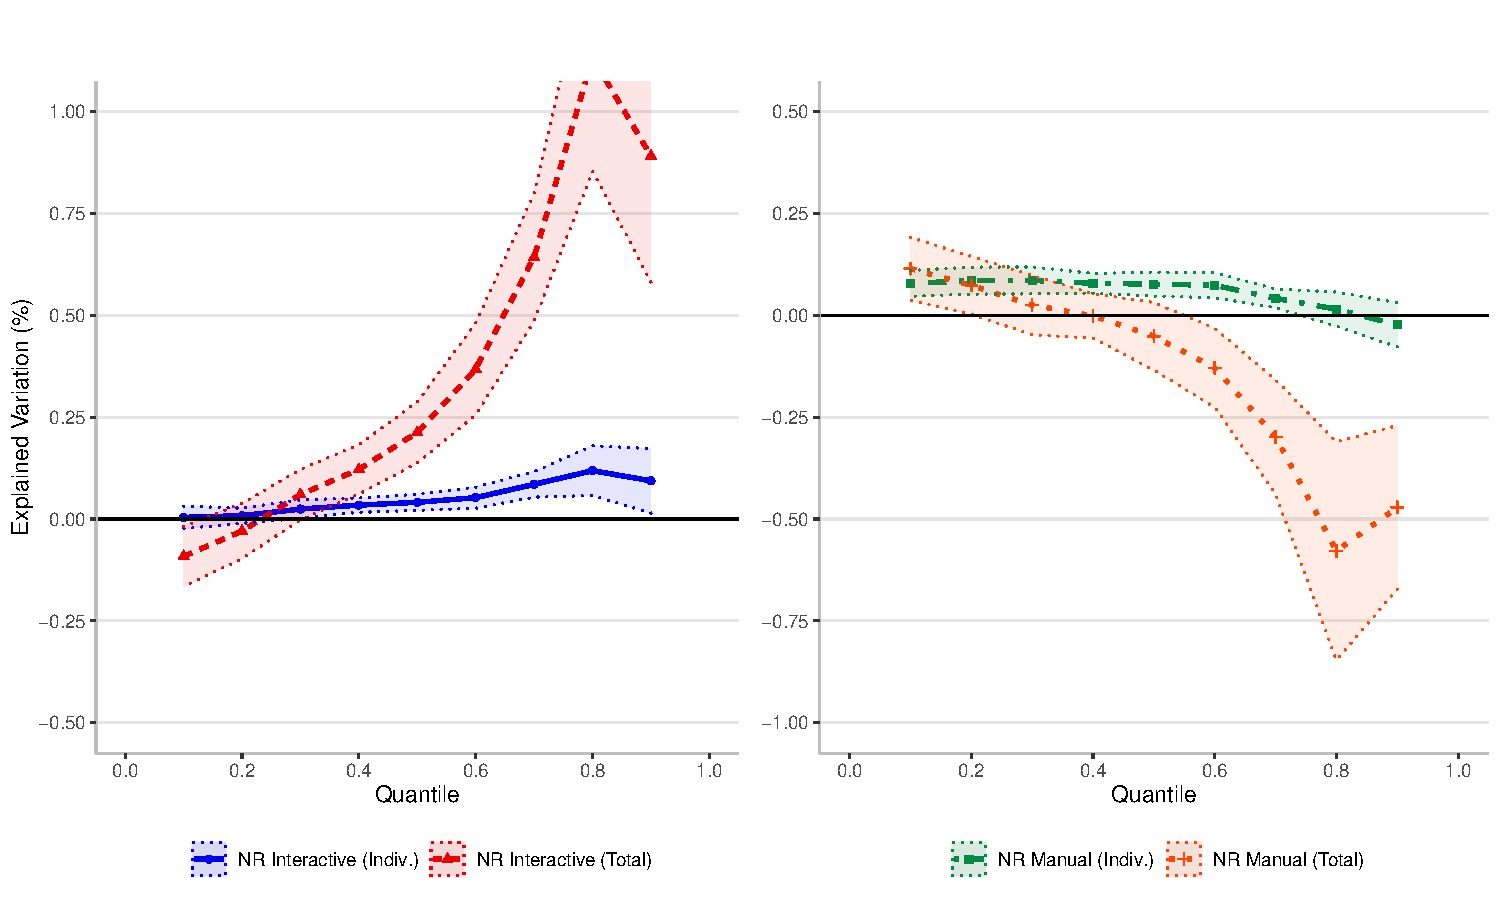
\includegraphics[scale=0.3]{rif_base_nri_nrm} \\
%			{\footnotesize \tiny NOTE. \textemdash The decomposition results are top-censored for clarity, i.e. cut off at contributions of (+-) 100\% to the explained wage gap. \\ Point estimates are displayed with a 95\% Confidence Interval. \par}
%			\caption{\centering Contributions of Individual-level variation in Tasks to the explained Native-Foreign Wage Gap, 1992-2018 \label{fig:wgap_indiv_occ}}
%		\end{minipage}
%	\end{figure}
	
\begin{itemize} 
	\item $IOV_{NRI}^{0.9} = 0.12$
	\item $IOV_{NRM}^{0.1} = 2.2$ 
\end{itemize} 

\hyperlink{regression}{\beamergotobutton{Regression}}	
	
\end{frame}


%------------------------------------------------


%\begin{frame}
%	\frametitle{Key Results RIF Decomposition: Long-term Trends (Abstract Tasks)}


%\begin{figure}[H]
%			\begin{minipage}{0.95\textwidth} % choose width suitably
%				\centering
%	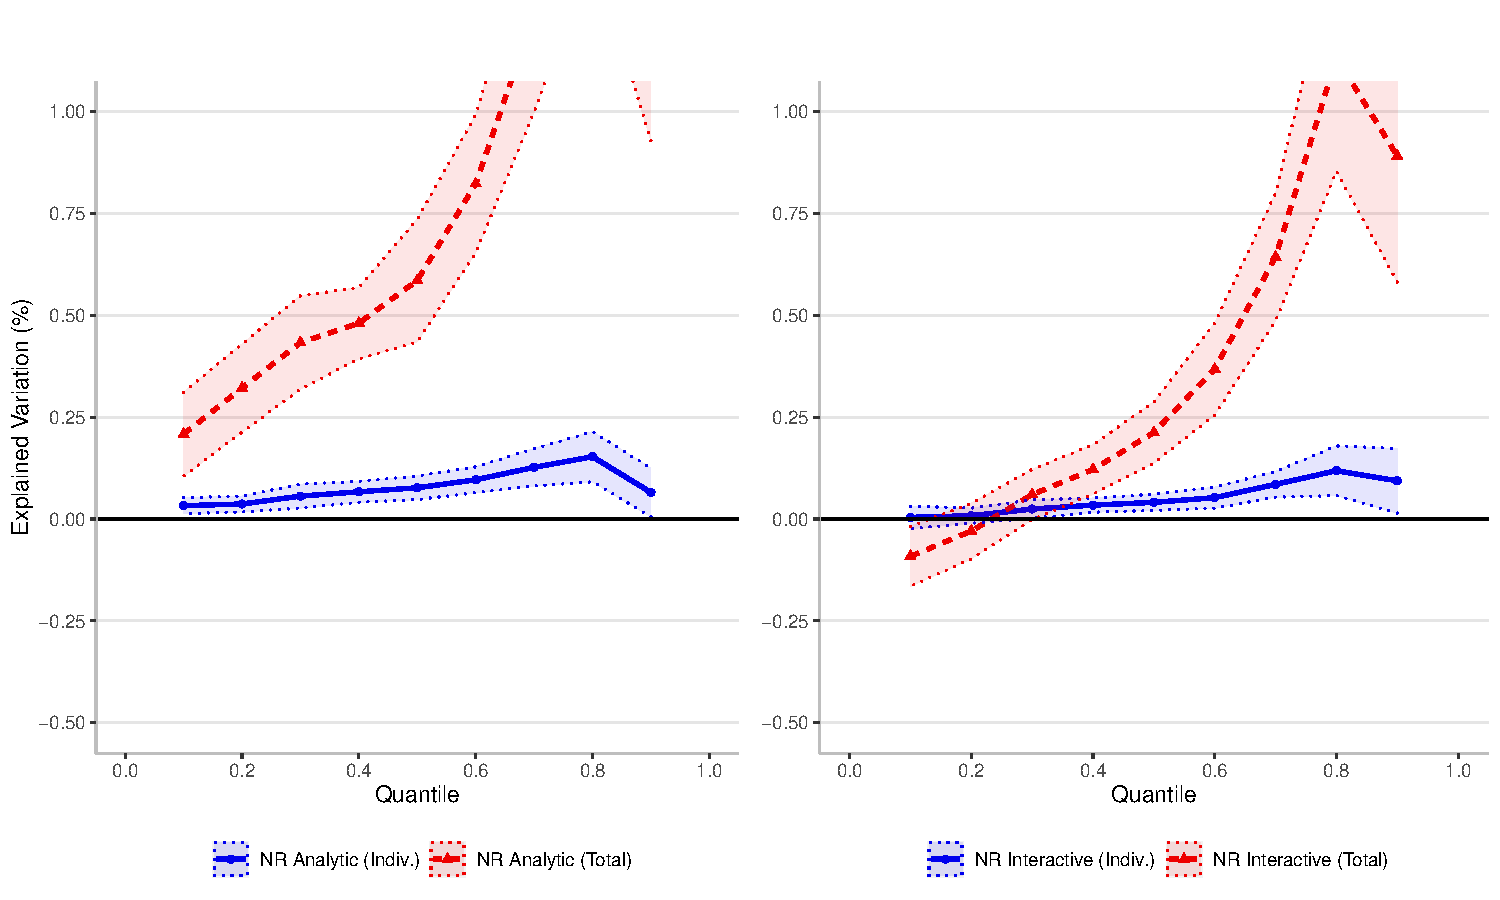
\includegraphics[scale=0.38]{rif_base_all_cog} \\
%	{\footnotesize \tiny NOTE. \textemdash The decomposition results are top-censored for clarity, i.e. cut off at contributions of 100\% to the explained wage gap.\par}
%	\caption{\centering Contributions of Individual-level variation in Abstract Tasks to the explained Native-Foreign Wage Gap, 1992-2018 \label{fig:wgap_indiv_occ}}
%		\end{minipage}
%\end{figure}


%\end{frame}


%------------------------------------------------


\begin{frame}[label=occ_spec] 
	\frametitle{Key Results RIF Decomposition: \\ Trends in  Occupational Segregation}
	
%	
%	\begin{figure}[H]
%		\begin{minipage}{0.95\textwidth} % choose width suitably
%			\centering
%			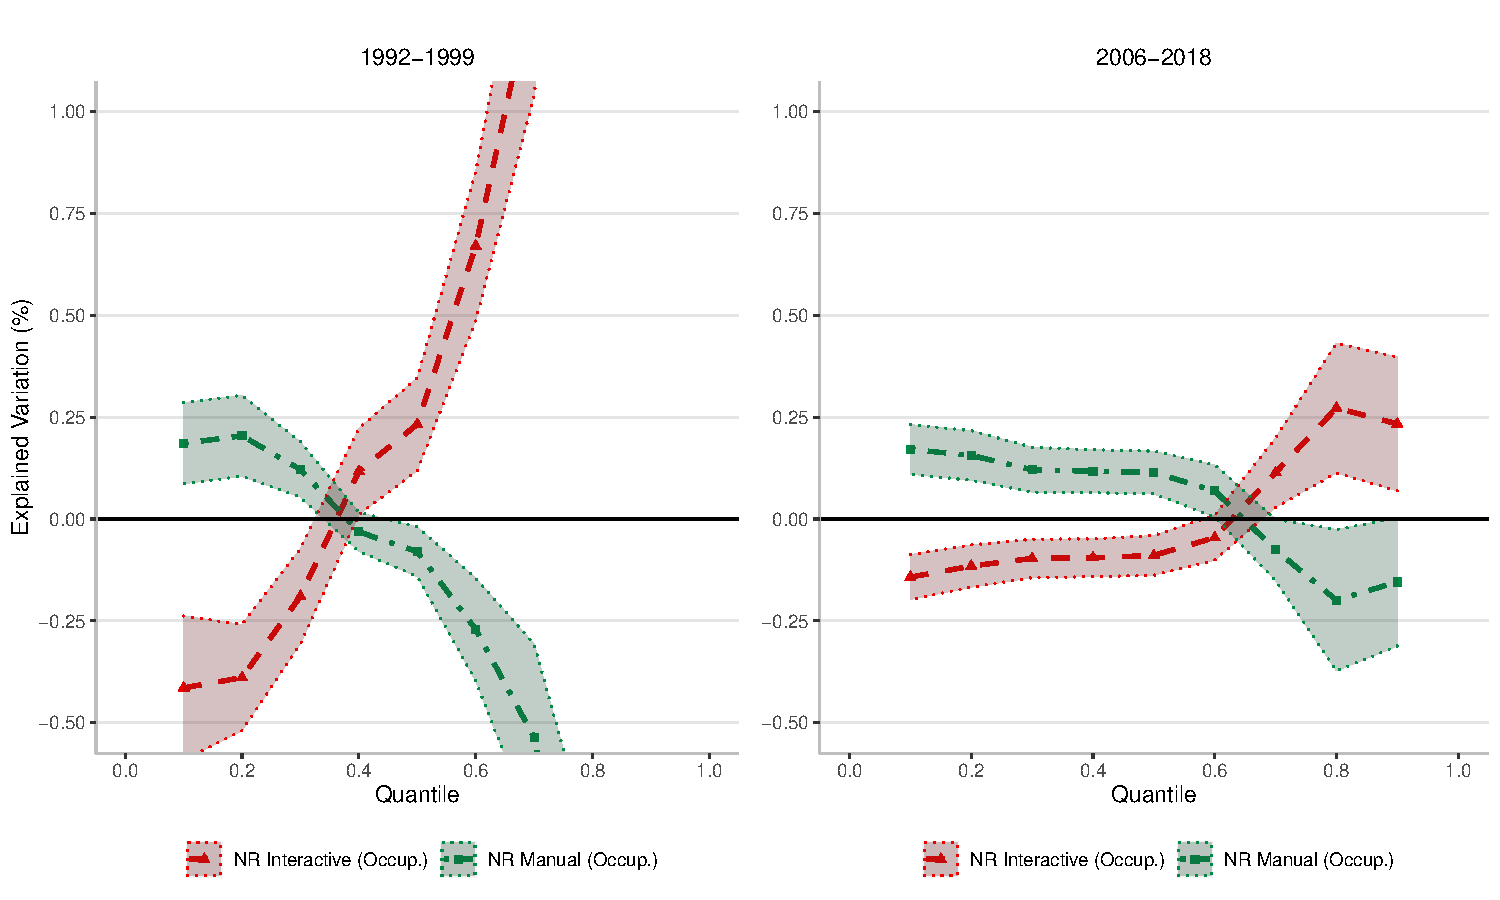
\includegraphics[scale=0.26]{rif_bw_nrinrm}
%			\caption{Contributions of Occup.-level variation in Tasks to the Wage Gap, 1992-2018 \label{fig:wgap_occ_seg} \label{fig:wage_gap_base}}
%			{\footnotesize \tiny NOTE. \textemdash The decomposition results are top-censored for clarity, i.e. cut off at contributions of 100\% \& -50\% to the explained wage gap. \\ Point estimates are displayed with a 95\% Confidence Interval. \par}
%			%{\caption  {Contributions of Task Variation Within Occupations to the explained Native-Foreign Wage Gap with base task group Routine Manual, 1992-2018 \label{fig:wgap_within_baserm}}}
%		\end{minipage}
%	\end{figure}
	
\begin{itemize} 
	\item Decline of economic significance of occupational segregation
\end{itemize} 

	\hyperlink{regression}{\beamergotobutton{Regression}}
		
\end{frame}


%------------------------------------------------


%\begin{frame}
%	\frametitle{Key Results RIF Decomposition: Evolution of Occupational Segregation - Manual Tasks}

%	\begin{figure}[H]
%				\begin{minipage}{0.95\textwidth} % choose width suitably
%					\centering
%		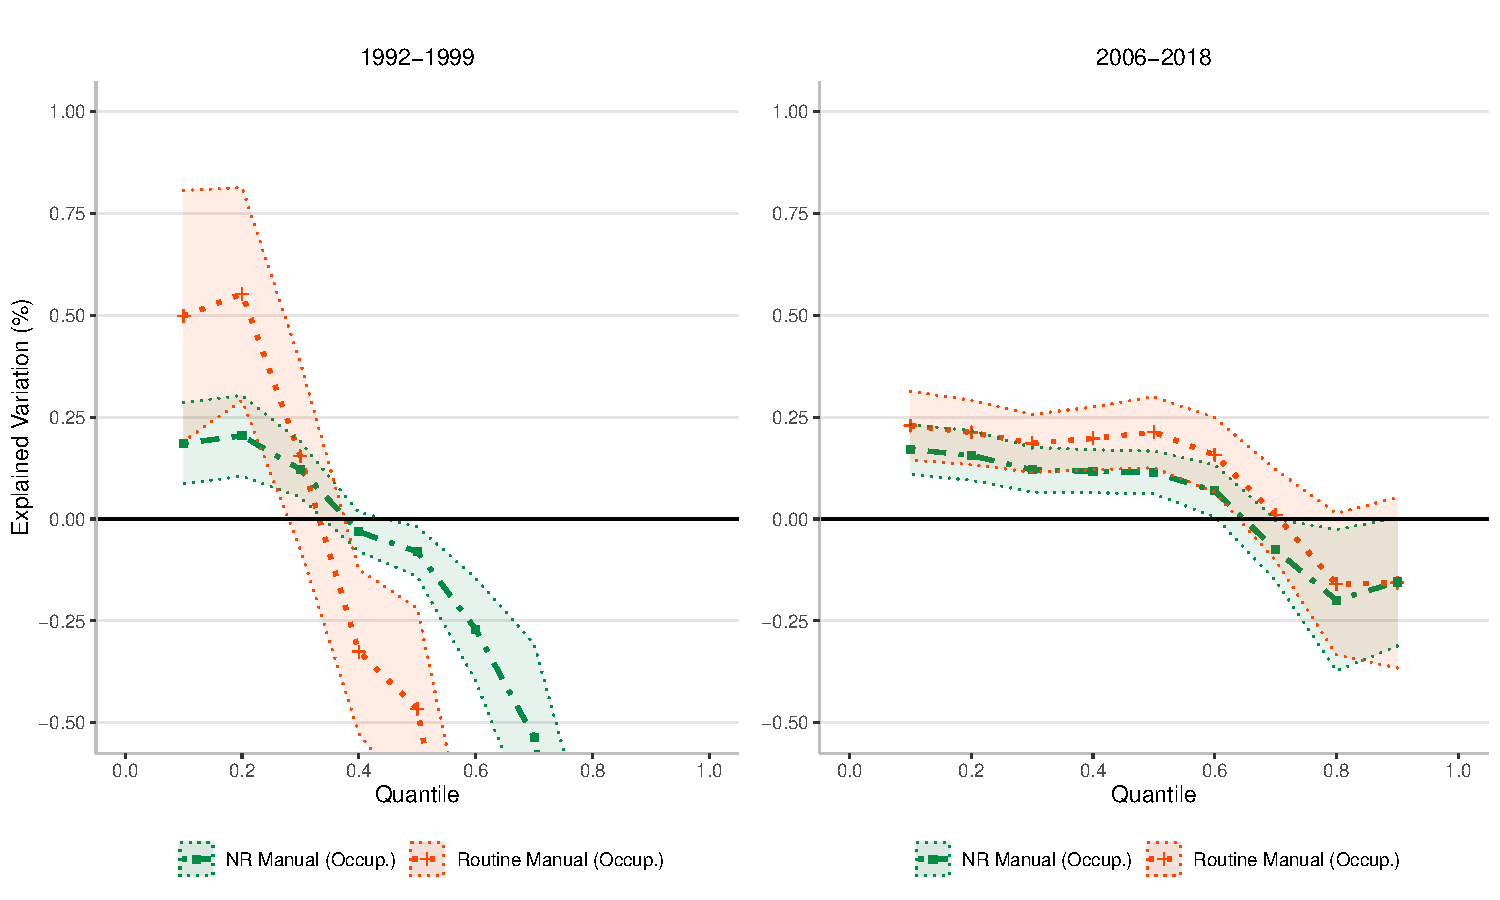
\includegraphics[scale=0.36]{rif_bw_man106}
%		\caption{Contributions of Individual-level variation in Tasks to the explained Wage Gap by Manual Tasks, 1992-2018 \label{fig:wgap_subs} \label{fig:wage_gap_base}}
%			{\footnotesize \tiny NOTE. \textemdash The decomposition results are top-censored for clarity, i.e. cut off at contributions of -50\% to the explained wage gap. \\ Point estimates are displayed with a 95\% Confidence Interval. \par}
%{\caption  {Contributions of Task Variation Within Occupations to the explained Native-Foreign Wage Gap with base task group Routine Manual, 1992-2018 \label{fig:wgap_within_baserm}}}
%				\end{minipage}
%	\end{figure}

%	\medskip

%	\begin{itemize} 
%		\item Decline in economic significance of occupational segregation
%	\end{itemize} 

%\end{frame}


%------------------------------------------------
\begin{frame}[label=wi_spec] 
	\frametitle{Assessment of Relative Importance of Within-Occupation Task Specialization}
	
	
%	Note:
	
%	\begin{itemize}
%		\item $\Delta T_{j, \tau} = \Delta T_{j, \tau}^{I} + \Delta T_{j, \tau}^{O}$
%	\end{itemize}
	
%	\bigskip
	
	Compare the ratio of individual task variation relative to occupational FE ($IFEV$) in $j$ at $\tau$: 
	
	\begin{equation} \label{ifev}
	IFEV_{j}^{\tau} = \frac{\Delta T_{j, \tau}^{I}}{\Delta FE_{j, \tau}}  
	\end{equation}
	
	\bigskip
	
	Example: $IFEV_{NRI}^{0.8} = 1$
	
	\medskip
	
	$\Longrightarrow$ Individual variation in tasks equally important to occupational characteristics  
	
	
\end{frame}

%------------------------------------------------

\begin{frame}
	\frametitle{Key Results RIF Decomposition: \\ Trends in Within-Occupation Task Specialization}
	
%	\begin{figure}[H]
%		\begin{minipage}{0.95\textwidth} % choose width suitably
%			\centering
%			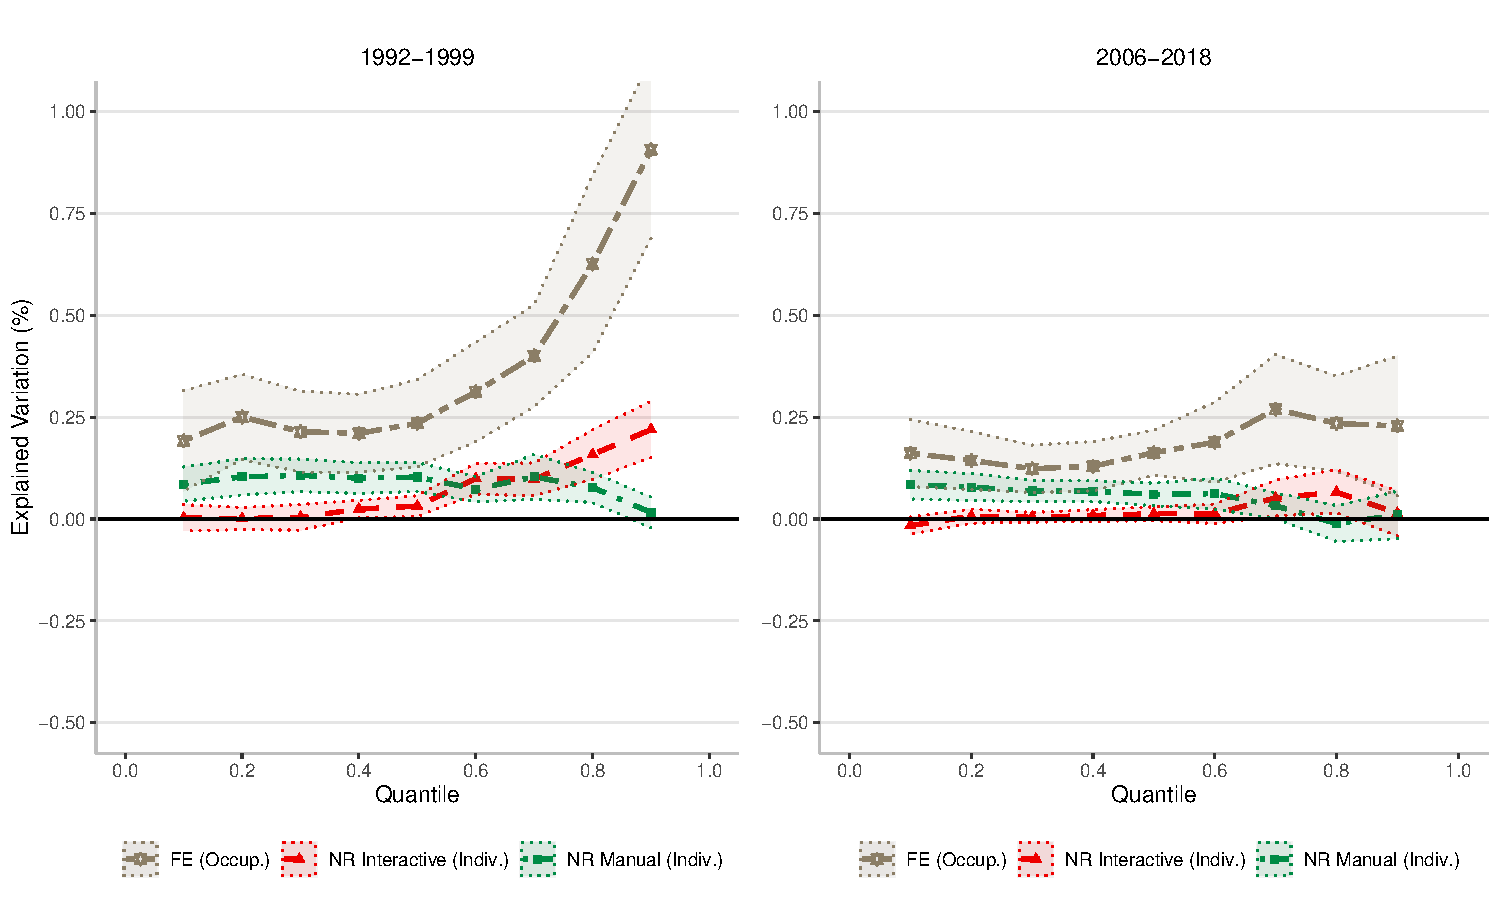
\includegraphics[scale=0.26]{rif_wi_nrinrm}
%			\caption{Contributions of Individual-level variation in Tasks to the explained Wage Gap conditional on Occupational FE, 1992-2018  \label{fig:wgap_win}}
%			{\footnotesize \tiny NOTE. \textemdash  Point estimates are displayed with a 95\% Confidence Interval. \par}
%			%{\caption  {Contributions of Task Variation Within Occupations to the explained Native-Foreign Wage Gap with base task group Routine Manual, 1992-2018 \label{fig:wgap_within_baserm}}}
%		\end{minipage}
%	\end{figure}
	
\def\HS{\hspace{\fontdimen2\font}}

\begin{itemize} 
	\item $IFEV_{NRI, 92-99}^{0.8} = 0.25$ \HS\HS\HS\HS\HS $IFEV_{NRI, 06-18}^{0.8} = 0.3$
	\item $IFEV_{NRM, 92-99}^{0.1} = 0.45$ \HS\HS\HS
	 $IFEV_{NRM, 06-18}^{0.1} = 0.55$ 
\end{itemize} 

%\hyperlink{regression}{\beamergotobutton{Regression}}
	
\end{frame}


%------------------------------------------------


%\begin{frame}
%	\frametitle{Key Results RIF Decomposition: Within-Occupation Task Specialization - Manual Tasks}

%	\begin{figure}[H]
%				\begin{minipage}{0.95\textwidth} % choose width suitably
%					\centering
%		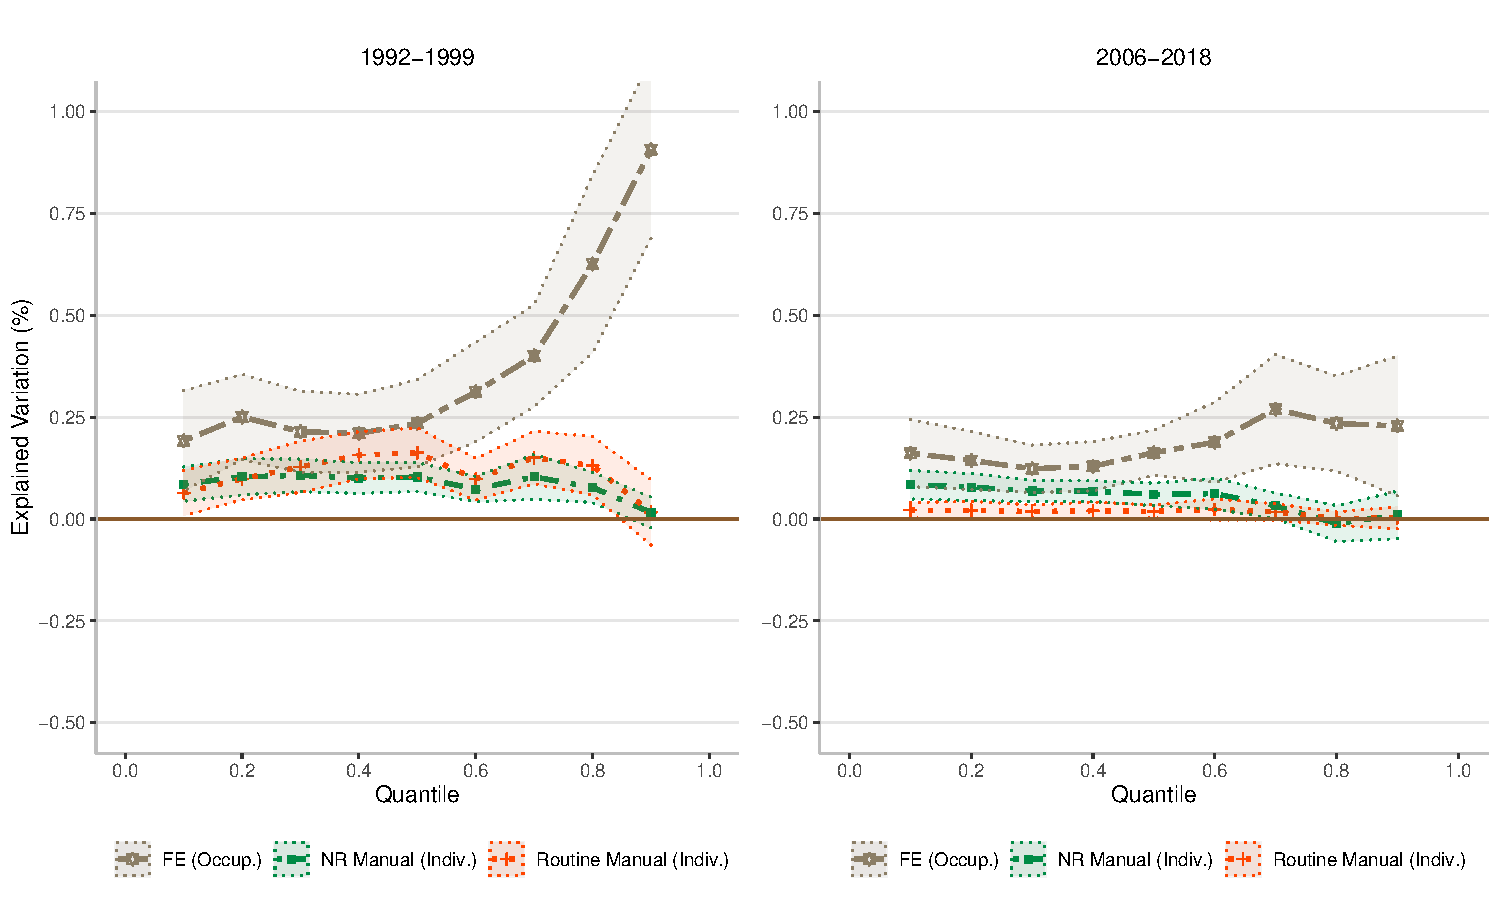
\includegraphics[scale=0.36]{rif_wi_man106}
%		\caption{Contributions of Individual-level variation in Tasks to the explained Wage Gap by Manual Tasks, 1992-2018 \label{fig:wgap_subs} \label{fig:wage_gap_base}}
%			{\footnotesize \tiny NOTE. \textemdash The decomposition results are top-censored for clarity, i.e. cut off at contributions of -50\% to the explained wage gap. \\ Point estimates are displayed with a 95\% Confidence Interval. \par}
%{\caption  {Contributions of Task Variation Within Occupations to the explained Native-Foreign Wage Gap with base task group Routine Manual, 1992-2018 \label{fig:wgap_within_baserm}}}
%				\end{minipage}
%	\end{figure}


%	\medskip

%	\begin{itemize} 
%		\item $IFEV_{NRI}^{0.8} (1992-99) = 0.2$ $\Longrightarrow$ $IFEV_{NRI}^{0.8} (2006-18) = 0.4$
%	\end{itemize} 

%\end{frame}


%------------------------------------------------


\begin{frame}
	\frametitle{Conclusions}
	
	\begin{enumerate}
		%\item \textbf{Native and Foreign Workers specialize in task assignments according to their comparative advantage}
		%	\begin{itemize}
		%	\item Natives specialize in abstract tasks involving problem-solving skills
		%	\item Foreigners specialize in manual tasks involving physical work
		%	\item Variation in interactive tasks has become an increasingly important determinant of the wage gap
		%	\item This trend is economically relevant within occupations, reinforcing already existing specialization patterns
		%	\item Future research should address differences in accumulation of human capital more formally \textbf{Bring Discusssion of Main Results in here}
		%	\end{itemize}
		%\medskip
		%
		\item \textbf{Task Specialization extends beyond occupational borders}
		\begin{itemize}
			\item Reinforces comparative advantage in interactive tasks among skilled labor, thus contributing to rising wage gap between N and F workers
			\item Structural models may understate LR wage \textit{gains} from immigration
		\end{itemize} 
		
		%Refined understanding for  small migration-induced wage effects: labor markets more segmented than previously assumed (key: incomplete transferability of human capital)
		
		\bigskip
		
		\item \textbf{Implications on Immigration Policy}
		\begin{itemize}
			\item Federal Recognition Act (2012) \& Skilled Immigration Act (2020) aim at improving recognition of foreign qualifications
			\item Findings suggest Policy Challenges with respect to 
				\begin{itemize}
					\item (i) Attraction \&
					\item (ii) Retention of skilled immigrant workers
				\end{itemize}
			%, but little success with programs involving occupation-specific skills
			%, especially of skilled foreign labor 
			
			%simplifies and standardizes procedures for the evaluation of foreign professional or vocational qualifications and opens up such procedures to target groups previously not entitled to pursue such a route, for example people from non-EU-countries. 
			
		\end{itemize} 
		
		
	\end{enumerate}
	
	
	
\end{frame}


%------------------------------------------------


\end{document}